\documentclass{standalone}
\usepackage{tikz}
\usetikzlibrary{patterns, positioning}
\usetikzlibrary{shapes.misc}
\usepackage[outline]{contour}
\contourlength{1.5pt} 
\usepackage[sfdefault]{ClearSans} %% option 'sfdefault' activates Clear Sans as the default text font
\usepackage[T1]{fontenc}

\begin{document}
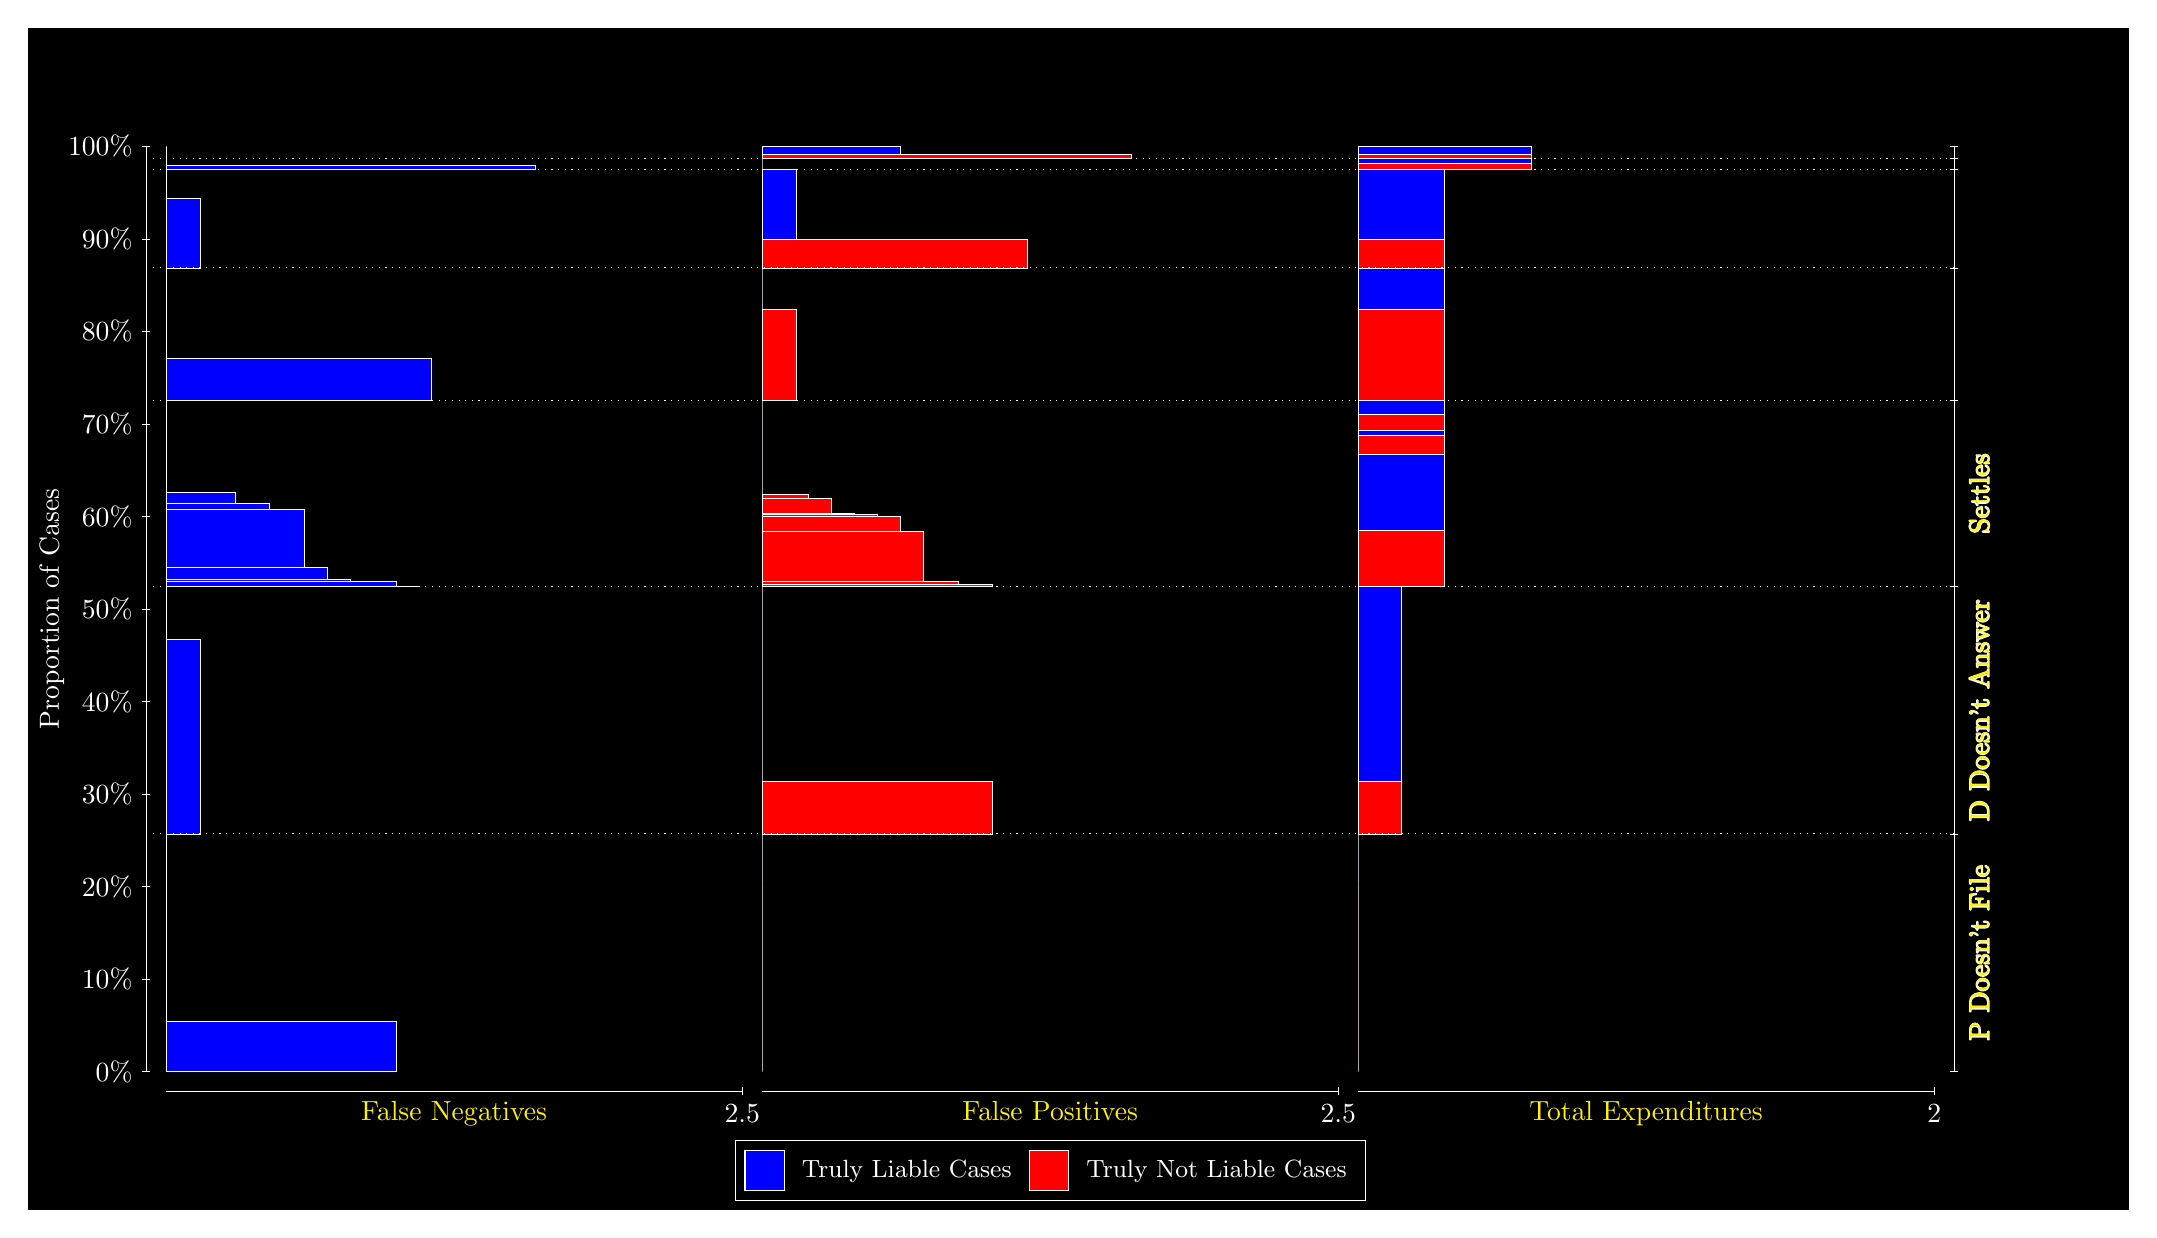
\begin{tikzpicture}
\draw[fill=black] (0,0) rectangle (26.667,15);
\draw[white, very thin] (1.5,1.75) -- (1.5,13.5);
\node[rotate=90, text=white, anchor=center] at (0.3, 7.625) {Proportion of Cases};
\draw[white, very thin] (1.45,1.75) -- (1.55,1.75);
\node[text=white, anchor=east] at (1.45, 1.75) {0\%};
\draw[white, very thin] (1.45,2.925) -- (1.55,2.925);
\node[text=white, anchor=east] at (1.45, 2.925) {10\%};
\draw[white, very thin] (1.45,4.1) -- (1.55,4.1);
\node[text=white, anchor=east] at (1.45, 4.1) {20\%};
\draw[white, very thin] (1.45,5.275) -- (1.55,5.275);
\node[text=white, anchor=east] at (1.45, 5.275) {30\%};
\draw[white, very thin] (1.45,6.45) -- (1.55,6.45);
\node[text=white, anchor=east] at (1.45, 6.45) {40\%};
\draw[white, very thin] (1.45,7.625) -- (1.55,7.625);
\node[text=white, anchor=east] at (1.45, 7.625) {50\%};
\draw[white, very thin] (1.45,8.8) -- (1.55,8.8);
\node[text=white, anchor=east] at (1.45, 8.8) {60\%};
\draw[white, very thin] (1.45,9.975) -- (1.55,9.975);
\node[text=white, anchor=east] at (1.45, 9.975) {70\%};
\draw[white, very thin] (1.45,11.15) -- (1.55,11.15);
\node[text=white, anchor=east] at (1.45, 11.15) {80\%};
\draw[white, very thin] (1.45,12.325) -- (1.55,12.325);
\node[text=white, anchor=east] at (1.45, 12.325) {90\%};
\draw[white, very thin] (1.45,13.5) -- (1.55,13.5);
\node[text=white, anchor=east] at (1.45, 13.5) {100\%};

\draw[white, very thin] (24.457,1.75) -- (24.457,13.5);
\draw[white, very thin] (24.407,1.75) -- (24.507,1.75);
\node[anchor=west] at (24.407, 1.75) {};
\draw[white, very thin] (24.407,4.7675) -- (24.507,4.7675);
\node[anchor=west] at (24.407, 4.7675) {};
\draw[white, very thin] (24.407,7.9073) -- (24.507,7.9073);
\node[anchor=west] at (24.407, 7.9073) {};
\draw[white, very thin] (24.407,10.274) -- (24.507,10.274);
\node[anchor=west] at (24.407, 10.274) {};
\draw[white, very thin] (24.407,11.956) -- (24.507,11.956);
\node[anchor=west] at (24.407, 11.956) {};
\draw[white, very thin] (24.407,13.204) -- (24.507,13.204);
\node[anchor=west] at (24.407, 13.204) {};
\draw[white, very thin] (24.407,13.343) -- (24.507,13.343);
\node[anchor=west] at (24.407, 13.343) {};
\draw[white, very thin] (24.407,13.5) -- (24.507,13.5);
\node[anchor=west] at (24.407, 13.5) {};

\draw[white, very thin, fill=blue] (1.75,1.75) rectangle (4.6775,2.3909);
\draw[white, very thin, fill=red] (1.75,2.3909) rectangle (1.75,4.7675);
\draw[white, very thin, fill=blue] (1.75,4.7675) rectangle (2.1891,7.2393);
\draw[white, very thin, fill=red] (1.75,7.2393) rectangle (1.75,7.9073);
\draw[white, very thin, fill=blue] (1.75,7.9073) rectangle (4.9703,7.918);
\draw[white, very thin, fill=blue] (1.75,7.918) rectangle (4.6775,7.9725);
\draw[white, very thin, fill=blue] (1.75,7.9725) rectangle (4.3848,7.981);
\draw[white, very thin, fill=blue] (1.75,7.981) rectangle (4.092,8.0002);
\draw[white, very thin, fill=blue] (1.75,8.0002) rectangle (3.7993,8.1545);
\draw[white, very thin, fill=blue] (1.75,8.1545) rectangle (3.5065,8.894);
\draw[white, very thin, fill=blue] (1.75,8.894) rectangle (3.0674,8.9729);
\draw[white, very thin, fill=blue] (1.75,8.9729) rectangle (2.6283,9.1027);
\draw[white, very thin, fill=red] (1.75,9.1027) rectangle (1.75,10.274);
\draw[white, very thin, fill=blue] (1.75,10.274) rectangle (5.1167,10.804);
\draw[white, very thin, fill=red] (1.75,10.804) rectangle (1.75,11.956);
\draw[white, very thin, fill=blue] (1.75,11.956) rectangle (2.1891,12.838);
\draw[white, very thin, fill=red] (1.75,12.838) rectangle (1.75,13.204);
\draw[white, very thin, fill=blue] (1.75,13.204) rectangle (6.4341,13.263);
\draw[white, very thin, fill=red] (1.75,13.263) rectangle (1.75,13.343);
\draw[white, very thin, fill=red] (1.75,13.343) rectangle (1.75,13.405);
\draw[white, very thin, fill=blue] (1.75,13.405) rectangle (1.75,13.5);
\draw[white, very thin, fill=red] (9.3189,1.75) rectangle (9.3189,4.1265);
\draw[white, very thin, fill=blue] (9.3189,4.1265) rectangle (9.3189,4.7675);
\draw[white, very thin, fill=red] (9.3189,4.7675) rectangle (12.246,5.4355);
\draw[white, very thin, fill=blue] (9.3189,5.4355) rectangle (9.3189,7.9073);
\draw[white, very thin, fill=red] (9.3189,7.9073) rectangle (12.246,7.9338);
\draw[white, very thin, fill=red] (9.3189,7.9338) rectangle (11.807,7.9714);
\draw[white, very thin, fill=red] (9.3189,7.9714) rectangle (11.368,8.6128);
\draw[white, very thin, fill=red] (9.3189,8.6128) rectangle (11.075,8.7957);
\draw[white, very thin, fill=red] (9.3189,8.7957) rectangle (10.783,8.8217);
\draw[white, very thin, fill=red] (9.3189,8.8217) rectangle (10.49,8.8387);
\draw[white, very thin, fill=red] (9.3189,8.8387) rectangle (10.197,9.0358);
\draw[white, very thin, fill=red] (9.3189,9.0358) rectangle (9.9044,9.0787);
\draw[white, very thin, fill=blue] (9.3189,9.0787) rectangle (9.3189,10.274);
\draw[white, very thin, fill=red] (9.3189,10.274) rectangle (9.758,11.426);
\draw[white, very thin, fill=blue] (9.3189,11.426) rectangle (9.3189,11.956);
\draw[white, very thin, fill=red] (9.3189,11.956) rectangle (12.686,12.321);
\draw[white, very thin, fill=blue] (9.3189,12.321) rectangle (9.758,13.204);
\draw[white, very thin, fill=red] (9.3189,13.204) rectangle (9.3189,13.284);
\draw[white, very thin, fill=blue] (9.3189,13.284) rectangle (9.3189,13.343);
\draw[white, very thin, fill=red] (9.3189,13.343) rectangle (14.003,13.405);
\draw[white, very thin, fill=blue] (9.3189,13.405) rectangle (11.075,13.5);
\draw[white, very thin, fill=red] (16.888,1.75) rectangle (16.888,4.1265);
\draw[white, very thin, fill=blue] (16.888,4.1265) rectangle (16.888,4.7675);
\draw[white, very thin, fill=red] (16.888,4.7675) rectangle (17.437,5.4355);
\draw[white, very thin, fill=blue] (16.888,5.4355) rectangle (17.437,7.9073);
\draw[white, very thin, fill=red] (16.888,7.9073) rectangle (17.986,8.6298);
\draw[white, very thin, fill=blue] (16.888,8.6298) rectangle (17.986,9.5865);
\draw[white, very thin, fill=red] (16.888,9.5865) rectangle (17.986,9.8265);
\draw[white, very thin, fill=blue] (16.888,9.8265) rectangle (17.986,9.8917);
\draw[white, very thin, fill=red] (16.888,9.8917) rectangle (17.986,10.101);
\draw[white, very thin, fill=blue] (16.888,10.101) rectangle (17.986,10.274);
\draw[white, very thin, fill=red] (16.888,10.274) rectangle (17.986,11.426);
\draw[white, very thin, fill=blue] (16.888,11.426) rectangle (17.986,11.956);
\draw[white, very thin, fill=red] (16.888,11.956) rectangle (17.986,12.321);
\draw[white, very thin, fill=blue] (16.888,12.321) rectangle (17.986,13.204);
\draw[white, very thin, fill=red] (16.888,13.204) rectangle (19.083,13.284);
\draw[white, very thin, fill=blue] (16.888,13.284) rectangle (19.083,13.343);
\draw[white, very thin, fill=red] (16.888,13.343) rectangle (19.083,13.405);
\draw[white, very thin, fill=blue] (16.888,13.405) rectangle (19.083,13.5);
\draw[white, dotted] (1.5,4.7675) -- (24.457,4.7675);
\draw[white, dotted] (1.5,7.9073) -- (24.457,7.9073);
\draw[white, dotted] (1.5,10.274) -- (24.457,10.274);
\draw[white, dotted] (1.5,11.956) -- (24.457,11.956);
\draw[white, dotted] (1.5,13.204) -- (24.457,13.204);
\draw[white, dotted] (1.5,13.343) -- (24.457,13.343);
\draw[white, very thin] (1.75,1.5) -- (9.0689,1.5);
\node[text=yellow, anchor=north] at (5.4094, 1.5) {False Negatives};
\draw[white, very thin] (9.0689,1.45) -- (9.0689,1.55);
\node[text=white, anchor=north] at (9.0689, 1.45) {2.5};

\draw[white, very thin] (9.3189,1.5) -- (16.638,1.5);
\node[text=yellow, anchor=north] at (12.978, 1.5) {False Positives};
\draw[white, very thin] (16.638,1.45) -- (16.638,1.55);
\node[text=white, anchor=north] at (16.638, 1.45) {2.5};

\draw[white, very thin] (16.888,1.5) -- (24.207,1.5);
\node[text=yellow, anchor=north] at (20.547, 1.5) {Total Expenditures};
\draw[white, very thin] (24.207,1.45) -- (24.207,1.55);
\node[text=white, anchor=north] at (24.207, 1.45) {2};

\node[text=yellow, centered, rotate=90] at (24.777, 3.2587) {\contour{white}{P Doesn't File}};
\node[text=yellow, centered, rotate=90] at (24.777, 6.3374) {\contour{white}{D Doesn't Answer}};
\node[text=yellow, centered, rotate=90] at (24.777, 9.0907) {\contour{white}{Settles}};





\draw (12.978300999999998,1.5) node[draw=none] (baseCoordinate) {};
\begin{scope}[align=center]
        \matrix[scale=0.5, draw=white, below=0.5cm of baseCoordinate, nodes={draw}, column sep=0.1cm]{
            \node[rectangle, draw, minimum width=0.5cm, minimum height=0.5cm, fill=blue] {}; &
            \node[draw=none, font=\small, text=white] (B) {Truly Liable Cases}; &
            \node[rectangle, draw, minimum width=0.5cm, minimum height=0.5cm, fill=red] {}; &
            \node[draw=none, font=\small, text=white] (B) {Truly Not Liable Cases}; \\
            };
\end{scope}

\end{tikzpicture}
\end{document}